\chapter{Model  for a  cooling elastic-plated  gravity
  current}
\label{chap3}
\minitoc

We present here  a general model, based on  the elastic-plated gravity
current  model developed  in  the  last section,  to  account for  the
cooling of the magmatic intrusion.

\section{Theory}
\label{C3-sec:theory}

\subsection{Formulation}
\label{C3-sec:formulation}

We model an axisymmetric fluid  blister of thickness $h(r,t)$ below an
elastic layer  of constant thickness  $d_c$ and above a  semi infinite
rigid layer \citep{Michaut:2011kg}  (Figure \ref{C3-sketch}) The fluid
is injected  continuously at the base  and center of the  blister at a
rate $Q(t)$  through a  conduit of  diameter $a$.  The hot  fluid is
intruded at temperature $T_i$ and cools through the top and the bottom
by conduction  in the surrounding  medium, whose temperature  $T_s$ is
allowed to increase with time.

\begin{figure}[htbp]
  \begin{center}
    \graphicspath{ {/Users/thorey/Documents/These/Manuscript/Figure/Chapter3/} }
    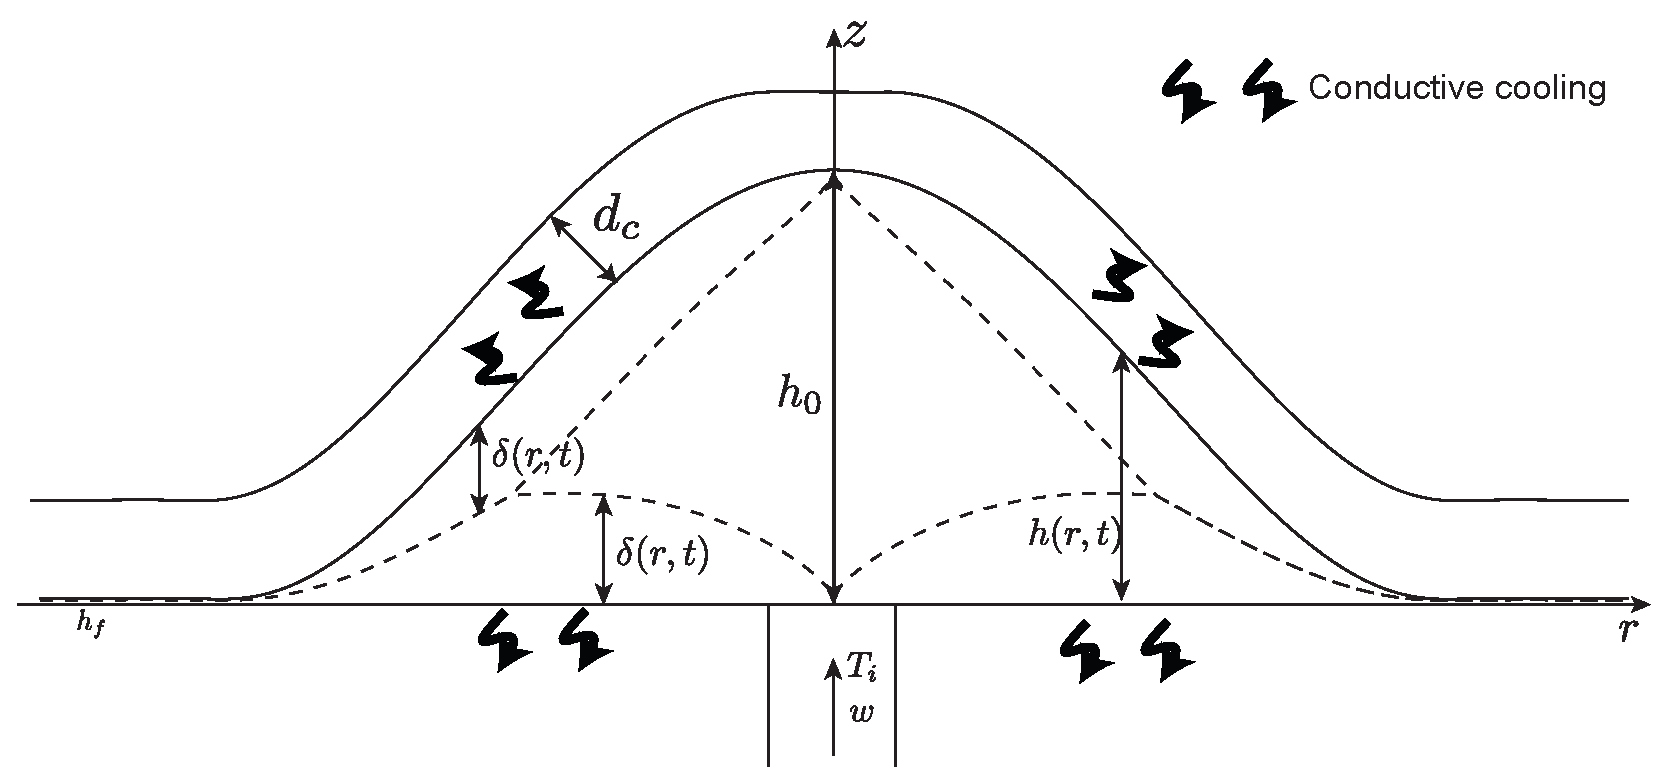
\includegraphics[scale=0.40]{C3-sketch.pdf}
    \caption{Model geometry and parameters.}
    \label{C3-sketch}
  \end{center}
\end{figure}

As  it  cools,  the  viscosity  of the  fluid  increases  following  a
prescribed  rheology   $\eta(T)$  bounded  between  two   values:  the
viscosity of the  hottest fluid $\eta_h$ at temperature  $T_i$ and the
viscosity of the coldest fluid $\eta_c$ at temperature $T_0$.

\subsection{Equation for the thickness}

For  a cooling  elastic-plated  gravity current,  the velocity  fields
depends   on   the   viscosity,    which   itself   depends   on   the
temperature. Without knowledge on the  form of the rheology $\eta(T)$,
integrating twice  (\ref{C2_V1}) using no-slip boundary  conditions at
the top and the bottom now gives
\begin{equation}
  u(r,z,t) = \frac{\partial P}{\partial r}\left(I(z)-I(h)\frac{z}{h}\right)
\end{equation}
with
\begin{equation}
  I(z) = \int_0^z\frac{z^*}{\eta(T)}dz^*
\end{equation}
where the driving pressure $P(r,z,t)$ is given by (\ref{C2-pression}).
However, instead of plugging in  this expression in (\ref{C2-Mass}) as
in  section   \ref{C2-sec:Governing  equation},  we   develop  another
approach which takes into account  the symmetry of the velocity around
$h/2$.  Indeed,  as we  will see  in the  next section,  this property
comes out naturally from the symmetry of the used vertical temperature
structure  which implies the same  symmetry for
the viscosity $\eta(T)$.

Integrating once (\ref{C2_V1})  as a function of z  using the symmetry
around $h/2$ gives
\begin{equation}
  \frac{\partial   u}{\partial   z}   =   \frac{1}{\eta}\frac{\partial
    P}{\partial r}\left(z-\frac{h}{2}\right)
\label{C3-deriv}
\end{equation}
and therefore, the velocity $u(r,z,t)$ reads
\begin{equation}
  u(r,z,t) = \frac{\partial P}{\partial r} I_0(z)
\end{equation}
with
\begin{equation}
  I_0(z) = \int_0^z\frac{1}{\eta(T)}\left(y-\frac{h}{2}\right)dy
\label{C3-I_0}
\end{equation}
Moreover, we have that
\begin{equation}
  \int_0^h u dz = -\int_0^h\frac{\partial u}{\partial z}zdz
\end{equation}
and therefore, the statement  of mass conservation (\ref{C2-Mass}) can
be written
\begin{eqnarray}
  \frac{\partial h}{\partial t} = \frac{1}{r}
  \frac{\partial}{\partial
  r} \left( r\int_0^h\frac{\partial u}{\partial z}zdz\right) + w_i
  \label{C3-Mass}
\end{eqnarray}
where we can now plug in (\ref{C3-deriv}) to finally obtain
\begin{eqnarray}
  \frac{\partial h}{\partial t} = \frac{1}{r}
  \frac{\partial}{\partial r} \left( r\left(\rho_m g \frac{\partial h}{\partial      r}+D\frac{\partial}{\partial      r}\left(\nabla^4h\right)\right)I_1(h)\right)
  + w_i.
  \label{C3-Mass-2}
\end{eqnarray}
with 
\begin{equation}
  I_1(z) = \int_0^z\frac{1}{\eta(T)}\left(y-\frac{h}{2}\right)ydy
\label{C3-I_1}
\end{equation}

\subsection{Heat transport equation}

\subsubsection{Local energy conservation}\\

In the laminar regime and in axisymmetrical coordinates ($r$,$z$), the
local energy  conservation equation within the  lubrication assumption
is written as
\begin{eqnarray}
  \frac{D}{D t}\left(\rho_m C_{p,m} T+\rho_mL(1-\phi)\right)&=& k_m  \frac{\partial^2
                                                                T}{\partial
                                                                z^2}
\label{C3-EnergyCons}
\end{eqnarray}

where  $T(r,z,t)$  is  the  fluid temperature,  $\phi(r,z,t)$  is  the
crystal fraction  in the melt  and $\rho_m$, $k_m$, $C_{p,m}$  and $L$
are the density,  thermal conductivity, specific heat  and latent heat
of the  fluid.  In this model,  the crystals are considered  only as a
source/sink of energy  as they melt/form during  the flow emplacement.
In particular, they share the same properties that the fluid itself.

Following a common approximation, we  assume that the crystal fraction
is a linear function of temperature over the melting interval
\begin{equation}
  \phi = \frac{T_L-T}{T_L-T_s}
  \label{C3-meltfraction}
\end{equation}
where $T_S$ and $T_L$ are the solidus and liquidus temperatures of the
magma  \citep{Hort:1997hk,Michaut:2006di}.   With this  approximation,
the local energy equation (\ref{C3-EnergyCons}) resumes to
\begin{eqnarray}
  \frac{\partial T}{\partial t}+ u\frac{\partial T}{\partial r}
  + w\frac{\partial T}{\partial z}  &=& \frac{ \kappa_m}{1+St^{-1}}  \frac{\partial^2
                                        T}{\partial               z^2}
                                        \label{C3-EnergyCons2}
\end{eqnarray}
where  $u(r,z,t)$ and  $w(r,z,t)$ are  the radial  and vertical  fluid
velocities,  $St  =\left(C_{p,m}(T_L-T_S)\right)/L$   is  the  Stephan
number   and    $\kappa_m$   is   the   fluid    thermal   diffusivity
$\kappa_m = k_m/\rho_m  C_{p,m}$.  Following \citet{BALMFORTH:2004fm},
we use an integral balance method to solve the heat transport equation
(\ref{C3-EnergyCons2}).   This theory  is based  on the  integral-balance
method of heat-transfer theory of \citet{Goodman:1958ue}, in which the
vertical structure of the temperature  field is represented by a known
function of depth that approximates the expected solution.

\subsubsection{Integral   balance   solution   for   the   temperature
  $T(r,z,t)$}

We model  the cooling of the  fluid blister through the  growth of two
thermal  boundary layers:  one growing  downward  from the  top and  a
second  growing upward  from  the base.   As  we consider  homogeneous
thermal properties for  the surrounding rocks, we assume  that the two
thermal boundary layers grow symmetrically and have the same thickness
$\delta(r,t)$.   In agreement,  the integral-balance  approximation we
use for the vertical temperature profile $T(r,z,t)$ is
\begin{equation}
  T=
  \begin{cases}
    T_b - (T_b-T_s)(1-\frac{z}{\delta})^2 & 0 \le z\le \delta \\
    T_b & \delta \le z\le h-\delta \\
    T_b - (T_b-T_s)(1-\frac{h-z}{\delta})^2 & h-\delta \le z\le h\\
  \end{cases}
  \label{C3-Temperature}
\end{equation}
where $T_b(r,t)$  is the  temperature at  the center  of the  flow and
$T_s(r,t)$ the temperature  at the contact with  the surrounding rocks
(Figure   \ref{Figure2-1}).    The   integral  balance   solution   in
(\ref{C3-Temperature}) assumes  a symmetry around $z=h/2$  and a decrease
of the  temperature in  the two  thermal boundary  layers down  to the
surrounding  rock  temperature   $T_s$  \citep{BALMFORTH:2004fm}.   In
addition,  it  assumes a  uniform  temperature  $T_b$ in  between  the
thermal  boundary  layers.   Then,  as  the fluid  is  injected  at  a
temperature  $T_i$,   we  have  $T_b(r,t)  =T_i$   when  $\delta<h/2$.
However,   if  the   two   thermal  boundary   layers  connect,   then
$\delta = h/2$ and $T_b$ decreases such that $T_b\le T_i$.

\subsubsection{Integral balance equation}
\label{C3-sec:integr-balance-equat}

We   begin    by   integrating    the   local    energy   conservation
(\ref{C3-EnergyCons2})  over  the  two   thermal  boundary  layers.   The
integration over the  bottom thermal layer, i.e. from  the base, $z=0$
to a level $z = \delta$ gives
\begin{eqnarray}
  &&\frac{\partial}{\partial t}\left( \delta( \bar{T}-T_b)\right)+\frac{1}{r}\frac{\partial}{\partial r} \left( r\delta(\overline{uT}-\bar{u}T_b)\right) + \delta\left( \frac{\partial T_b}{\partial t}+ \overline{u}\frac{\partial T_b}{\partial r}\right)\nonumber\\
  &=&-\frac{\kappa_m}{1+St^{-1}}\left. \frac{\partial T}{\partial z}\right|_{z=0}+w_{i}(T_{i}-T_b)
      \label{C3-Local1}
\end{eqnarray}
where the  bar indicate the  vertical average over the  bottom thermal
boundary layer
\begin{equation}
  \overline{f} = \frac{1}{\delta}\int_0^{\delta}f dz\nonumber,
\end{equation}
$T_b(r,t)$  is  the temperature  at  $z=\delta$,  $w_{i}(r)$ is  the
vertical  injection velocity  and  we  have used  the  nullity of  the
thermal gradient at $z=\delta$ and the local mass conservation
\begin{equation}
  \frac{1}{r}\frac{\partial ru}{\partial r} +\frac{\partial w}{\partial z}=0.
  \label{C3-MassConservation}
\end{equation}
The  integration over  the top  thermal layer,  i.e., from  the level,
$z=h-\delta$ to the top $z=h$ gives:
\begin{eqnarray}
  &&\frac{\partial}{\partial t}\left( \delta( \bar{T}-T_b)\right)+\frac{1}{r}\frac{\partial}{\partial r} \left( r\delta(\overline{uT}-\bar{u}T_b)\right) + \delta\left(\frac{\partial T_b}{\partial t}+ \overline{u}\frac{\partial T_b}{\partial r}\right)\nonumber\\
  &=&\frac{\kappa_m}{1+St^{-1}}\left. \frac{\partial T}{\partial z}\right|_{z=h}.
      \label{C3-Local2}
\end{eqnarray}
where,    in    addition    to    the    local    mass    conservation
(\ref{C3-MassConservation})  and   the  fact  the  thermal   gradient  at
$z=h-\delta$ is  equal to  zero, we have  used the  kinematic boundary
condition in $z=h(r,t)$
\begin{equation}
  \frac{\partial h}{\partial t} +u\frac{\partial h}{\partial
    r} = w
\end{equation}
The heat balance equation can then be written by adding (\ref{C3-Local1})
and (\ref{C3-Local2}) and introducing (\ref{C3-Temperature})
\begin{eqnarray}
  &&\frac{\partial}{\partial t}\left( \delta( \bar{T}-T_b)\right)+\frac{1}{r}\frac{\partial}{\partial r} \left( r\delta(\overline{uT}-\bar{u}T_b)\right) + \delta\left( \frac{\partial T_b}{\partial t}+ \overline{u}\frac{\partial T_b}{\partial r}\right)\nonumber\\
  &=&\frac{\kappa_m}{2(1+St^{-1})}\left(\left. \frac{\partial T}{\partial z}\right|_{z=h}-\left. \frac{\partial T}{\partial z}\right|_{z=0}\right)+\frac{w_{i}}{2}(T_{i}-T_b)
      \label{C3-LocalHeat3}
\end{eqnarray}

\subsubsection{Thermal boundary conditions}
\label{C3-sec:thermal-boundary-condition}

At  the  contact with  the  surrounding  rock,  the  heat is  lost  by
conduction:
\begin{equation}
  k_m\left.\frac{\partial                                    T}{\partial
      z}\right|_{z=0}=k_r\left.\frac{\partial              T_r}{\partial
      z}\right|_{z=0}
  \label{C3-Flux1}
\end{equation}
\begin{equation}
  k_m\left.\frac{\partial                                  T}{\partial
      z}\right|_{z=h}=k_r\left.\frac{\partial            T_r}{\partial
      z}\right|_{z=h}
  \label{C3-Flux2}
\end{equation}

where  $T_r(r,z)$  is  the  temperature  in  the  surrounding  medium.
Assuming  a  semi  infinite  layer  for  the  rigid  layer  below  the
intrusion, \citet{Carslaw:1959wf}  show that the temperature  $T_r$ in
the surrounding rocks can be approximated to a first order by
\begin{equation}
  T_r(r,z,t)-T_0=(T_{s}-T_0)\operatorname{erfc}{\left(\frac{-z}{2\sqrt{\kappa_r t}}\right)}.
  \label{eq22}
\end{equation}
The  thickness of  the upper  layer is  equal to  the intrusion  depth
$d_c$. However,  we assume that the  depth $d_c$ is large  compared to
the characteristic  length scale for  conduction $L_c$ and we  use the
same approximation to derive $T_r$ above the intrusion
\begin{equation}
  T_r(r,z,t)-T_0=(T_{s}-T_0)\operatorname{erfc}{\left(\frac{z-h}{2\sqrt{\kappa_r t}}\right)}.
  \label{eq11}
\end{equation}
Therefore,  the  two  thermal boundary  conditions  (\ref{C3-Flux1})  and
(\ref{C3-Flux2}) become:
\begin{equation}
  k_m\left.\frac{\partial                                    T}{\partial
      z}\right|_{z=0}= k_r
  \frac{T_{s}-T_{0}}{\sqrt{\pi \kappa_r t}}
  \label{C3-Flux_1}
\end{equation}
\begin{equation}
  k_m\left.\frac{\partial                                    T}{\partial
      z}\right|_{z=h}= -k_r
  \frac{T_{s}-T_{0}}{\sqrt{\pi \kappa_r t}}
  \label{C3-Flux_2}
\end{equation}


\subsection{Dimensionless equations}
\label{C3-sec:dimens-equat}

We   first    rewrite   the    different   temperatures    such   that
$T=T_0+\left(T_i-T_0)\theta$ where  $\theta(r,z,t)$ is  the equivalent
  dimensionless  temperature.   In  term  of  $\theta$,  the  integral
  balance approximation (\ref{C3-Temperature}) rewrites
  \begin{equation}
    \theta(z)=
    \begin{cases}
      \Theta_b -\left(\Theta_b-\Theta_s\right)(1-\frac{z}{\delta})^2& 0 \le z\le \delta \\
      \Theta_b & \delta \le z\le h-\delta \\
      \Theta_b -\left(\Theta_b-\Theta_s\right)(1-\frac{h-z}{\delta})^2
      & h-\delta \le z\le h
    \end{cases}
    \label{Temperature2}
  \end{equation}
  where            $\Theta_b=\frac{T_b-T_0}{T_{i}-T_0}$            and
  $\Theta_s        =       \frac{T_s-T_0}{T_i-T_0}$.         Equations
  (\ref{C3-LocalHeat3})  and  (\ref{C3-Mass})  are  nondimensionalized
  using the same horizontal scale $\Lambda$, vertical height scale $H$
  and time  scale $\tau$ used is  section \ref{C2-sec:dimens-equat} as
  well        as       a        horizontal       velocity        scale
  $U=\Lambda/\tau=\left(\rho_m          g          H^3\right)/\left(12
    \eta_h\Lambda\right)$ to give
  \begin{eqnarray}
    \frac{\partial h}{\partial t}& =& \frac{12}{r}
                                      \frac{\partial}{\partial r} \left( r\left( \frac{\partial h}{\partial      r}+\frac{\partial}{\partial      r}\left(\nabla^4h\right)\right)I_1(h)\right)
                                      + w_i\label{EqFinal1}\\
    \frac{\partial}{\partial
    t}\left( \delta( \bar{\theta}-\Theta_b)\right)&=&-\frac{1}{r}\frac{\partial}{\partial
                                                      r}  \left(   r\delta(\overline{u\theta}-\bar{u}\Theta_b)\right)  -
                                                      \delta\left(      \frac{\partial       \Theta_b}{\partial      t}+
                                                      \overline{u}\frac{\partial     \Theta_b}{\partial    r}\right)\nonumber\\
                                 &-&
                                     2Pe^{-1}St_m\frac{\left(\Theta_b-\Theta_s\right)}{\delta}+\frac{w_{i}}{2}(1-\Theta_b)\label{HeatDimensionLess}\\
    u(r,z,t)&   =&   12\left(   \frac{\partial   h}{\partial
                   r}+\frac{\partial}{\partial
                   r}\left(\nabla^4h\right)\right)I_0(z)\label{C3-Veloc}\\
    w_{i}&=&
             \frac{32}{\gamma^{2}}\left(\frac{1}{4}-\frac{r^{2}}{\gamma^{2}}\right)\left(1-\frac{h_0}{\sigma}\right)\hspace{.2cm}
             \text{if} \hspace{.2cm} r < \gamma/2 \\
\end{eqnarray}
with 
\begin{eqnarray}
  I_0(z)&=&\int_0^z\frac{1}{\eta(\theta,\nu)}\left(y-\frac{h}{2}\right)
    dy \\
I_1(z) &=& \int_0^z\frac{1}{\eta(\theta,\nu)}\left(y-\frac{h}{2}\right)y dy
  \end{eqnarray}
  where $\eta(\theta,\nu)$ is the dimensionless rheology $\eta/\eta_h$
  which  depends on  the  dimensionless temperature  $\theta$ and  the
  dimensionless  number  $\nu$.   In addition,  the  thermal  boundary
  conditions (\ref{C3-Flux_1}) and (\ref{C3-Flux_2}) resume to
  \begin{equation}
    2\frac{\Theta_b-\Theta_s}{\delta}               =               \Omega
    Pe^{1/2}\frac{\Theta_s}{\sqrt{\pi t}}.
    \label{C3-Boundary-Condi}
  \end{equation}
  $\gamma$, $\sigma$,  $Pe$, $St_m$,  $\nu$ and  $\Omega$ are  the six
  dimensionless numbers that control the dynamics of the flow
  \begin{eqnarray}
    \gamma&=&\frac{a}{\Lambda} \label{gamma}\\
    \sigma &=& \frac{\Delta P}{\rho_m g h_0} \label{sigma}\\
    Pe&=& \frac{H^2}{\kappa_m \tau}\label{Pe}\\
    St_m &=& \frac{C_{p,m}\left(T_L-T_S\right)}{C_{p,m}\left(T_L-T_S\right)+L} \label{St}\\
    \nu&=& \frac{\eta_h}{\eta_c}\label{nu}\\
    \Omega&=&\frac{k_r}{k_m}\left(\frac{\kappa_m}{\kappa_r}\right)^{1/2}\label{omega}
  \end{eqnarray}
  $\gamma$ is the dimensionless radius  of the conduit and $\sigma$ is
  the normalized  pressure head which  have been discussed  in section
  \ref{C2-sec:model}.   $Pe$ is  the  Peclet number,  it compares  the
  vertical  diffusion  of heat  to  the  horizontal advection  in  the
  intrusion interior. $St_m$  is a modified Stephan number,  it is the
  ratio of  sensible heat  between solidus and  liquidus to  the total
  energy of  the fluid at liquidus  temperature and tends to  one when
  the  crystallization is  neglected. $\nu$  is the  maximum viscosity
  contrast, i.e.  the ratio between the hottest and coldest viscosity.
  $\Omega$ is  the ratio between  heat conduction at the  contact with
  the encasing rocks and heat diffusion within the fluid.

  \subsection{Further simplifications}
  \label{C3-sec:furth-simpl}

  \textbf{Heat balance equation} \vspace{.5cm}

  The heat balance equations (\ref{HeatDimensionLess}) can reduce to
  \begin{eqnarray}
    \frac{\partial}{\partial
    t}\left( \delta( \bar{\theta}-1)\right)+\frac{1}{r}\frac{\partial}{\partial
    r}
    \left( r\delta(\overline{u\theta}-\bar{u})\right)&=&- 2Pe^{-1}St_m\frac{\left(\Theta_b-\Theta_s\right)}{\delta} 
                                                         \label{HeatD_a}
  \end{eqnarray}

  Indeed, if the thermal boundary layers exist, $\Theta_b=1$, $\delta$
  is    the     variable    and    the    heat     balance    equation
  (\ref{HeatDimensionLess}) reduces  to the  equation (\ref{HeatD_a}).
  In contrast, if the thermal  boundary layers merge, $\delta=h/2$ and
  the variable is $\Theta_b$. In this case, the heat balance equations
  (\ref{HeatDimensionLess}) reduces to:
  \begin{eqnarray}
    \frac{\partial h\bar{\theta}}{\partial t}+\frac{1}{r}\frac{\partial}{\partial
    r} \left( rh\overline{u\theta}\right)-\Theta_b\left(\frac{\partial h}{\partial t}+\frac{1}{r}\frac{\partial}{\partial
    r} \left( rh\bar{u}\right)\right)&=& - 8St_mPe^{-1}\frac{\left(\Theta_b-\Theta_s\right)}{h}+w_{i}(1-\Theta_b)\nonumber
  \end{eqnarray}
  which we can rewrite using (\ref{EqFinal1}) as
  \begin{equation}
    \frac{\partial h\bar{\theta}}{\partial t}+\frac{1}{r}\frac{\partial}{\partial
      r} \left( rh\overline{u\theta}\right) &=& w_i
    - 8St_mPe^{-1}\frac{\left(\Theta_b-\Theta_s\right)}{h}\nonumber\\
  \end{equation}
  which  also  corresponds  to   (\ref{HeatD_a})  in  the  case  where
  $\delta=h/2$.

  Following \citet{BALMFORTH:2004fm}, we rewrite (\ref{HeatD_a}) using
  a new variable $\xi = \delta(1-\overline{\theta})$
  \begin{equation}
    \frac{\partial \xi}{\partial t}+\frac{1}{r}\frac{\partial}{\partial r} \left( r\bar{u}\xi\right)-\frac{1}{r}\frac{\partial}{\partial r} \left( r\delta(\overline{u\theta}-\bar{u}\bar{\theta})\right)&=&2Pe^{-1}St_m\frac{\left(\Theta_b-\Theta_s\right)}{\delta}
    \label{EqFinal2}
  \end{equation}
  The second term of the equation contains advection by the vertically
  integrated  radial   velocity  while  the  third   term  contains  a
  correction accounting for the  vertical structure of the temperature
  field. The term  on the right is  the loss of heat  by conduction in
  the surrounding medium.

  \vspace{.5cm} \textbf{Average quantities} \vspace{.5cm}

  The average  velocity over  a thermal boundary  layer $\overline{u}$
  reads
  \begin{eqnarray}
    \overline{u}        =\frac{1}{\delta}\int_0^{\delta}udz        &=&
                                                                       u(r,\delta,t) - \frac{1}{\delta}\int_0^{\delta}\frac{\partial
                                                                       u}{\partial z} zdz\\
                                                                   &=&\frac{12}{\delta}
                                                                       \frac{\partial
                                                                       P}{\partial
                                                                       r}\left(\delta
                                                                       I_0(\delta)-I_1(\delta)\right)
  \end{eqnarray}
  where $P(r,z,t) = h+\nabla^4h$ is  the dimensionless pressure and we
  have     used    (\ref{C3-Veloc}).      The    average     advection
  $\overline{u\theta}$ over a thermal boundary layer reads
  \begin{eqnarray}
    \overline{u\theta}=\frac{1}{\delta}\int_0^{\delta}u\theta dz &=& \frac{1}{\delta}\left( [ uG(z) ]_{0}^{\delta} -\int_0^\delta
                                                                     G(z)\frac{\partial
                                                                     u}{\partial
                                                                     z}
                                                                     dz\right)\nonumber\\
                                                                 &=&\frac{12}{\delta} \frac{\partial P}{\partial r}\left(G(\delta)I_0(\delta)-I_2(\delta)\right)
  \end{eqnarray}
  where
  \begin{equation}
    G(z)                  =                 \Theta_b                  z
    -\frac{\left(\Theta_b-\Theta_s\right)}{3}\delta\left(1-\frac{z}{\delta}\right)^3
  \end{equation}
  denotes a primitive of $\theta$ when $z<\delta$ and
  \begin{equation}
    I_2(z)=\int_0^y                         \frac{1}{\eta(\theta,\nu)}G(y)
    \left(y-\frac{h}{2}\right)dy.
  \end{equation}
  Therefore, we have
  \begin{equation}
    \overline{u\theta}-\overline{u}\overline{\theta}= \frac{12}{\delta} \frac{\partial P}{\partial r}\left(I_0(\delta)\left(G(\delta)-\delta\overline{\theta}\right)+\overline{\theta}I_1(\delta)-I_2(\delta)\right)
  \end{equation} 
  where the average temperature over a thermal boundary layer reads
  \begin{equation}
    \overline{\theta} = \frac{2}{3}\left( \Theta_{b}+\Theta_{s}\right)
    \label{C3-tbar}
  \end{equation}

  \vspace{.5cm} \textbf{Main variables} \vspace{.5cm}

  The variable  $\xi$ is the sufficient  variable to solve for  in the
  heat transport equation (\ref{EqFinal2}). Indeed,
  \begin{equation}
    \xi&=&\frac{\delta}{3} \left(- 2 \Theta_{b} - \Theta_{s} + 3\right)\label{C3-xi}
  \end{equation}
  where   we   have   used   (\ref{C3-tbar}).    In   addition,   from
  (\ref{C3-Boundary-Condi}), we can rewrite
  \begin{eqnarray}
    \Theta_s &=& \frac{2 \Theta_{b}}{\beta \delta + 2}\label{C3-Ts},\\
    \delta  &=&   \frac{1}{\Theta_{s}  \beta}   \left(2  \Theta_{b}   -  2
                \Theta_{s}\right)\label{C3-D},\\
    \Theta_b &=& \frac{\Theta_{s}}{2} \left(\beta \delta + 2\right)\label{C3-Tb}
  \end{eqnarray}
  where $\beta = \Omega Pe^{1/2}/\sqrt{\pi t}$ for clarity.

  When  the thermal  boundary  layer just  merged, then  $\Theta_b=1$,
  $\delta = h/2$ and injecting (\ref{C3-Ts})  into (\ref{C3-xi}) gives
  \begin{equation}
    \xi_t(t)=\frac{\beta(t) h^{2}{\left (r,t \right )}}{6 \beta(t) h{\left (r,t \right )}
      + 24}\label{C3-xit}
  \end{equation}

  Therefore,  when $\xi<\xi_t$,  the  thermal boundary  layer are  not
  merged, $\Theta_b=1$  and injecting (\ref{C3-D})  into (\ref{C3-xi})
  and solving for $\Theta_s$ gives
  \begin{equation}
    \Theta_s = \frac{3 \beta}{4} \xi - \frac{\sqrt{3}}{4} \sqrt{\beta \xi \left(3 \beta \xi + 8\right)} + 1.
  \end{equation}
  
  In  contrast,  when  $\xi>\xi_t$,  the thermal  boundary  layer  are
  merged, $\delta=h/2$ and  injecting (\ref{C3-Tb}) into (\ref{C3-xi})
  and solving for $\Theta_s$ gives
  \begin{equation}
    \Theta_s = \frac{- 12 \xi + 6 h}{\left(\beta h + 6\right) h}.
  \end{equation}

  \subsection{Summary of the equations}

  The  equation governing  the  cooling of  an elastic-plated  gravity
  current with rheology $\eta(\theta,\nu)$ are summarized as follow
  \begin{eqnarray}
    \frac{\partial h}{\partial t}-\frac{12}{r}
    \frac{\partial}{\partial      r}
    \left(      r      I_1(h)\left(     \frac{\partial      }{\partial
    r}\left(h+\nabla^4h\right)\right)\right)
\label{C3-HF}
    & =& w_i\\
    \frac{\partial                                       \xi}{\partial
    t}+\frac{1}{r}\frac{\partial}{\partial                          r}
    \left( r\left(\bar{u}\xi-\Sigma\right)\right)&=&2Pe^{-1}St_m\frac{\left(\Theta_b-\Theta_s\right)}{\delta}\label{C3-TF}
  \end{eqnarray}
  where
  \begin{equation}
    \Theta_s(r,t)=
    \begin{cases}
      \frac{3 \beta}{4} \xi - \frac{\sqrt{3}}{4} \sqrt{\beta \xi \left(3 \beta \xi + 8\right)} + 1 & \text{if} \hspace{1cm} \xi\leq \xi_t \\
      \frac{- 12 \xi + 6 h{\left (r,t \right )}}{\left(\beta h{\left (r,t \right )} + 6\right) h{\left (r,t \right )}} & \text{if} \hspace{1cm} \xi > \xi_t\\
    \end{cases}
\label{C3-TS}
  \end{equation}
  \begin{equation}
    \Theta_b(r)=
    \begin{cases}
      1 &\text{if } \hspace{1cm} \xi\leq \xi_t \\
      \frac{\Theta_{s}}{4} \left(\beta(t) h{\left (r,t \right )} +
        4\right) & \text{if} \hspace{1cm} \xi > \xi_t\\
    \end{cases}
\label{C3-TB}
  \end{equation}
  \begin{equation}
    \delta(r)=
    \begin{cases}
      \frac{1}{\Theta_{s} \beta(t)} \left(- 2 \Theta_{s} + 2\right) &\text{if } \hspace{1cm} \xi\leq \xi_t \\
      h(r,t)/2 & \text{if} \hspace{1cm} \xi > \xi_t\\
    \end{cases}
\label{C3-DELTA}
  \end{equation}
  with
  \begin{eqnarray}
    \xi_t(t)&=&\frac{\beta(t) h^{2}{\left (r,t \right )}}{6 \beta(t) h{\left (r,t \right )}
                + 24}\\
    \beta(t) &=& \Omega Pe^{1/2}\frac{1}{\sqrt{\pi t}}\\
    \overline{u}&=& \frac{12}{\delta}
                    \left( \frac{\partial }{\partial r}\left(h+\nabla^4h\right)\right)\left(\delta
                    I_0(\delta)-I_1(\delta)\right)\\
                    \Sigma     &=&12   \left( \frac{\partial }{\partial r}\left(h+\nabla^4h\right)\right)\left(I_0(\delta)\left(G(\delta)-\delta\overline{\theta}\right)+\overline{\theta}I_1(\delta)-I_2(\delta)\right)\\
    \overline{\theta}                                              &=&
                          \frac{2}{3}\left( \Theta_{b}+\Theta_{s}\right)\\
    G(z)              &    = &                \Theta_b                  z
    -\frac{\left(\Theta_b-\Theta_s\right)}{3}\delta\left(1-\frac{z}{\delta}\right)^3\\
w_i&=&\frac{32}{\gamma^{2}}\left(\frac{1}{4}-\frac{r^{2}}{\gamma^{2}}\right)\left(1-\frac{h_0}{\sigma}\right)
  \end{eqnarray}
and
\begin{eqnarray}
  I_0(z)&=&\int_0^z\frac{1}{\eta(\theta,\nu)}\left(y-\frac{h}{2}\right)
    dy \\
I_1(z) &=& \int_0^z\frac{1}{\eta(\theta,\nu)}\left(y-\frac{h}{2}\right)y dy\\
    I_2(z)&=&\int_0^y                         \frac{1}{\eta(\theta,\nu)}
    \left(y-\frac{h}{2}\right)G(y)dy.\\
\end{eqnarray}


\section{Numerical approach}
\label{C3-sec:numerical-approach}

\subsection{General procedure}
\label{sec:general-procedure}

The coupled nonlinear partial differential equations (\ref{C3-HF}) and
(\ref{C3-TF}) are solved on a grid of size $M$ defined by the relation
$r_i = (i-0.5)\Delta r$ for $i=1,..,M$. The grid is shifted at the center to avoid
problem arising  from the axisymmetrical  geometry. We index  the grid
point by the indice $i$ and denote the solution on this grid $h_i$ and
$\xi_i$ and the secondary variables $\Theta_{b,i}$, $\Theta_{s,i}$ and
$\delta_i$. Both equations can be expressed on the convenient form
\begin{equation}
  \frac{\partial u}{\partial t} - f = 0
\end{equation}
where $u$  is the function we  want to integrate and  $f$ a non-linear
function  that depends  on $u$.   We  solve these  equations by  first
discretizing all the spatial  derivatives using Finite Difference. The
accuracy of the  scheme is determined by the  higher order derivatives
since  their numerical  approximation requires  the largest  number of
sample points. We then get  two systems of $M$ ordinary differential
equations with the form
\begin{equation}
  \frac{\partial u_i}{\partial t} - f_i = 0 \hspace{1cm} i = 1,...,M
\end{equation}
The time derivatives are first  order and, since explicit schemes tend
to be  very sensitive and unstable,  we use a fully  implicit backward
Euler scheme to get
\begin{equation}
  \frac{u_i^{n+1}-u_i^n}{\Delta t} - f_i(u_i^{n+1}) = 0 \hspace{1cm} i
  = 1,...,M
\label{C3-Num-1}
\end{equation}
Since  $f_i(u_i^{n+1})$ is  not a  linear function,  the system  above
cannot be re-arranged to solve $u_i^{n+1}$ in term of $u_i^{n}$ and an
iterative method  has to  be employed  instead. Fixed  point iteration
method have shown  poor results in converging toward  the solution and
we finally apply  second order Newton's method to  obtain the solution
at each time step.  In particular, we first linearize $u^{n+1}$ around
a guess  of the solution  by assuming $u^{n+1}=u^*+\delta  u^n$, where
$u^*$ is a guess and $\delta u^n$ is the error and we drop the $i$ for
clarity.   Then, we  expressed the  non-linear part  using a  Taylor's
expansion
\begin{equation}
  f^{n+1}=f(u^{n+1})=f(u^*+\delta
  u^n)=f(u^*)+J^h_{f}(u^*)\delta u^n\nonumber
\end{equation}
where  $J^u_{f}(u^*)$ is  the  jacobian matrix  for  the function  $f$
evaluated  in $h^*$.   Injecting the  expansion into  (\ref{C3-Num-1})
finally gives a  system of M linear equations for  the correction term
$\delta_h^n$ which can be expressed as
\begin{equation}
  (I-\Delta tJ^u_{f}(u^*))\delta u^n=u^n-u^*+\Delta t f(u^*)
\end{equation}
where $I$ is the identity matrix. Therefore,  each iteration solves  for $\delta u^n$  and we
use $u_n+\delta u^n$  as a new guess $u^*$ in  each iteration. This is
repeated  until $\delta  u^n$  becomes  sufficiently small.   Finally,
since the equations are coupled, we use a fixed-point iteration method
to  converge  toward  the  solution   $(h,\xi)$  at  each  time  step.
Therefore, the algorithm is the following at each time step
\begin{itemize}
\item Start with a guess for the values of all variables.
\item Solve the thickness equation (\ref{C3-HF}) for $h^{n+1}$ using Newton-Rhapsod method.
\item Solve the heat equation (\ref{C3-TF}) for $\xi^{n+1}$ using $h^{n+1}$ as a new guess for $h^*$
  and Newton-Rhapsod method.
\item Repeat  step one until  further iterations cease to  produce any
  significant changes in the values of both $h^{n+1}$ and $\xi^{n+1}$.
\end{itemize}
The computational scheme is summarized in the following.

\subsection{Thickness equation}

The thickness equation (\ref{C3-HF}) is written as
\begin{eqnarray}
  \frac{\partial h}{\partial t}-f(h,\xi)&=&0
\end{eqnarray}
with
\begin{eqnarray}
  f& =& \frac{1}{r}
        \frac{\partial}{\partial      r}
        \left(      r  \phi\left(     \frac{\partial      }{\partial
        r}\left(h+P\right)\right)\right)+w_i\\
  \phi &=& 12I_1(h)
\end{eqnarray}
and where $P$ is the dimensionless bending pressure $P = \nabla^4h$.

\vspace{.5cm} \textbf{Spatial discretization of f} \vspace{.5cm}

The  spatial discretization  is  obtained using  a central  difference
scheme  over  a  sub-grid  shifted  by $0.5\Delta  r$  from  the  main
grid. Therefore, we have
\begin{eqnarray}
  f_i&=&\frac{1}{r_i \Delta_r}\left(r_{i+1/2}\phi_{i+1/2}\left.\left(\frac{\partial h}{\partial r}+\frac{\partial P}{\partial r}\right)\right|_{i+1/2}-r_{i-1/2}\phi_{i-1/2}\left.\left(\frac{\partial h}{\partial r}+\frac{\partial P}{\partial r}\right)\right|_{i-1/2}\right)\nonumber\\
     &=&A_i\phi_{i+1/2}\left(h_{i+1}-h_i\right)-B_i\phi_{i-1/2}\left(h_{i}-h_{i-1}\right)\nonumber\\
     &+&A_i\phi_{i+1/2}\left(P_{i+1}-P_i\right)-B_i\phi_{i-1/2}\left(P_{i}-P_{i-1}\right)\nonumber\\
     &+&w_i\label{C3-Num-3}
\end{eqnarray}
where                $A_i=r_{i+1/2}/(r_i\Delta_r^2)$               and
$B_i=r_{i-1/2}/(r_i\Delta_r^2)$.   The bending  pressure  term $P$  is
very stiff and  needs a careful treatment.  In  particular, the fourth
order derivative requires a fourth order central difference scheme and
therefore, $P_i$ is  expressed over a seven point stencil  on the main
grid such that
\begin{equation}
  P_{i}=   \alpha_{i}h_{i-3}  +   \beta_{i}h_{i-2}+\gamma_{i}  h_{i-1}
  +\lambda_{i}h_{i}+\kappa_{i}h_{i+1}+\delta_ih_{i+2}+\epsilon_ih_{i+3}
  \label{C3-Num-4}
\end{equation}
with
\begin{eqnarray}
  &\alpha_{i}&=\frac{1}{24\Delta r^{4}}\left(-4+3p_3\Delta_r \right)\nonumber \\
  &\beta_{i}&=\frac{1}{24\Delta r^{4}}\left(48-24p_3\Delta_r-2p_2\Delta_r^2+2p_1\Delta_r^3\right) \nonumber\\
  &\gamma_{i}&=\frac{1}{24\Delta r^{4}}\left(-156+39p_3\Delta_r+32p_2\Delta_r^2-16p_1\Delta_r^3\right)\nonumber\\
  &\lambda_{i}&=\frac{1}{24\Delta r^{4}}\left(224-60p_2\Delta r^{2}\right) \nonumber\\
  &\kappa_{i}&=\frac{1}{24\Delta r^{4}}\left( -156-39p_3\Delta_r+32p_2\Delta_r^2+16p_1\Delta_r^3\right)\nonumber\\
  &\delta_{i}&=\frac{1}{24\Delta r^{4}}\left( 48+24p_3\Delta_r-2p_2\Delta_r^2-2p_1\Delta_r^3\right) \nonumber\\
  &\epsilon_{i}&=\frac{1}{24\Delta r^{4}}\left(-4-3p_3\Delta_r \right)\nonumber
\end{eqnarray}
and where $p_1=1/r_i^3$, $p_2=1/r_i^2$ and $p_3 = 2/r_i$. Finally, the
term $\phi_{i-1/2}$  and $\phi_{i-1/2}$, which depend  on the variable
$\Theta_b$, $\delta$ as well as  different power of $h$, are evaluated
in $i-1/2$ and  $i+1/2$ respectively. Different choices  for the value
of the variable at the mid-cell grid point do not show any significant
difference  and a  simple  average  is taken  such  that the  variable
$u_{i+1/2}$ is taken as $0.5(u_i+u_{i+1})$.

\vspace{.5cm}    \textbf{Expression   of    the   jacobian    $J_f^h$}
\vspace{.5cm}

The discretized  function $f_i$ can be  break down in three  part, the
gravitational part $f_i^{g}$  which is expressed in term  of the value
of $h$ on three  grid points $\left\{{i-1,i,i+1}\right\}$, the bending
part $f_i^{b}$ which is expressed in term  of the value of $h$ on nine
grid points  $\left\{{i-4,i-3,...,i+3,i+4}\right\}$ and  the injection
term which depends only on the grid point $i$ such that
\begin{equation}
  f_i = f_i^g+f_i^b+w_i
\end{equation}
Therefore, the jacobian is  nona-diagonal and its coefficient $J_{il}$
are
\begin{equation}
  J_{il}=
  \begin{cases}
    \frac{\partial f^{b}_i}{\partial h_{l}} &
    l = \left\{{i-4,i-3,i-2,i+2,i+3,i+4}\right\}\\
    \frac{\partial       f^{g}_i}{\partial       h_{l}}+\frac{\partial
      f^{b}_i}{\partial h_{l}} & l =
    \left\{{i-1,i,i+1}\right\}\\
    0 & \text{otherwise}
  \end{cases}
  \label{C2-eq12}
\end{equation}
The different  terms can be  easily derived from  (\ref{C3-Num-3}) and
(\ref{C3-Num-4}) with just slight  adjustment coming from the boundary
conditions.

\vspace{.5cm} \textbf{Boundary condition} \vspace{.5cm}

 We begin with
$h_i=h_f$ for  $i=1,..,M$.  Since the  flow is symmetric in  $r=0$, we
require that
\begin{equation}
  \left.\frac{\partial h}{\partial r}\right|_{r=0} =\left.\frac{\partial P}{\partial r}\right|_{r=0} =0
\end{equation}
and therefore for $i=1$, we have
\begin{eqnarray}
  f_i     &=&A_1\phi_{i+1/2}\left(h_{i+1}-h_i\right)\nonumber\\
          &+&A_i\phi_{i+1/2}\left(P_{i+1}-P_i\right)\nonumber\\
          &+&w_i\label{C3-Num-5}
\end{eqnarray}
The expression  of the  bending pressure, evaluated  over a  $7$ point
stencils, is problematic close to the boundary and reflection formulae
will  be  used  in  order   to  accommodate  the  boundary  conditions
\citet{Patankar:1980vu}.   In   particular,  we  have  $h_0   =  h_1$,
$h_{-1}=h_2$ and  $h_{-2}=h_3$.  Similarly, boundary condition  at the
end of the mesh is accounted by using a grid much larger than the flow
itself and requiring
\begin{equation}
  \left.\frac{\partial h}{\partial r}\right|_{r=r_M} =\left.\frac{\partial P}{\partial r}\right|_{r=r_M} =0
\end{equation}
which gives for $i=M$
\begin{eqnarray}
  f_i     &=&B_i\phi_{i-1/2}\left(h_{i}-h_{i-1}\right)\nonumber\\
          &+&B_i\phi_{i-1/2}\left(P_{i}-P_{i-1}\right)\nonumber\\
          &+&w_i\label{C3-Num-5}
\end{eqnarray}
with $h_{i>=M}=h_f$.


\vspace{.5cm} \textbf{Newton-Rhapsod method} \vspace{.5cm}

The Newton-Rhapsod method reads
\begin{equation}
  (I-\Delta tJ^h_{f}(h_k^*))\delta h_k^n=h^n-h_k^*+\Delta t f(h_k^*)
\end{equation}
where the  $k$ refers  to the $k$  iterations, $I$ is  a $M  \times M$
diagonal  matrix and  $J_f^h(h^*)$  is a  $M  \times M$  nona-diagonal
matrix.  This  system  of  linear  equations can  be  solved  using  a
nona-diagonal algorithm. At the first  iteration, we use $h^*_1 = h^n$
as     a    first     guess    and     then    we     iterate    using
$h^*_k  = h^n+\delta  h_{k-1}^n$ as  a new  guess for  each iterations
until $\delta h^n_{k}$ becomes  sufficiently small.  In particular, we
require that
\begin{equation}
  \delta h^n_k/h^*_{k}<\epsilon
\end{equation}
with $\epsilon = 10^{-4}$. 

\subsection{Heat equation}

The heat equation (\ref{C3-TF}) is written as
\begin{eqnarray}
  \frac{\partial \xi}{\partial t}-g(h,\xi)&=&0
\end{eqnarray}
with
\begin{eqnarray}
  g& =& \frac{1}{r}\frac{\partial}{\partial                          r}
        \left( r\Gamma\xi\right) +\frac{1}{r}\frac{\partial}{\partial                          r}
        \left(r\Sigma\right)+2Pe^{-1}St_m\frac{\left(\Theta_b-\Theta_s\right)}{\delta}\\
  \Gamma&=& -\overline{u}
\end{eqnarray}

\vspace{.5cm} \textbf{Spatial discretization of g} \vspace{.5cm}

As for the thickness equation,  the spatial discretization is obtained
using  a  central  difference  scheme   over  a  sub-grid  shifted  by
$0.5\Delta r$ from the main grid. Therefore, we have
\begin{eqnarray}
  g_i &=& \left(C_i\Gamma_{i+1/2}\xi_{i+1/2}-D_i\Gamma_{i-1/2}\xi_{i-1/2}\right)\\
      &+&\left(C_i\Sigma_{i+1/2}-D_i\Sigma_{i-1/2}\right)\\
      &+&2Pe^{-1}St_m\frac{\Theta_{b,i}-\Theta_{s,i}}{\delta_i}
\end{eqnarray}
with         $C_i         =r_{i+1/2}/(r_i\Delta        r)$         and
$D_i =r_{i-1/2}/(r_i\Delta r)$.   We use the average  between the grid
point $i$ and $i-1$ (resp. $i+1$) to evaluate the quantity in $\Gamma$
and  $\Sigma$ at  $i-1/2$ (resp.   $i+1/2$).   In addition,  we use  a
classical upwind  scheme to handle $\xi$  at the mid grid  point which
requires
\begin{eqnarray}
  \xi_{i+1/2} &=& \xi_i\\
  \xi_{i-1/2} &=& \xi_{i-1}
\end{eqnarray}

\vspace{.5cm}  \textbf{Expression   of  the   Jacobian  $J_{g}^{\xi}$}
\vspace{.5cm}

The expression  of the Jacobian  is much straightforward in  that case
and its coefficient $J_{il}$ are
\begin{equation}
  J_{il}=
  \begin{cases}
    -D_i\Gamma_{i-1/2}&
    l = i-1\\
    C_i\Gamma_{i+1/2} & l = i \\
    0 & \text{otherwise}
  \end{cases}
  \label{C2-eq12}
\end{equation}
with only slight adjustment coming from the boundary conditions.

\vspace{.5cm} \textbf{Boundary conditions} \vspace{.5cm}

We  consider $\Theta_b  =1$  and $\delta  = 10^{-4}$  in  the film  at
$t=0$. In this way, we ensure  that the average temperature across the
film at $t=0$ is close to $1$. By construction, $D_1=0$ and therefore,
for $i=1$ we have
\begin{eqnarray}
  g_i &=& C_i\Gamma_{i+1/2}\xi_{i}+ C_i\Sigma_{i+1/2} +2Pe^{-1}St_m\frac{\Theta_{b,i}-\Theta_{s,i}}{\delta_i}
\end{eqnarray}
For   $i=M$,   we    consider   that   $\Gamma_{i+1/2}=\Gamma_i$   and
$\Sigma_{i=1/2}=\Sigma_i$.   However,  the  choice  for  the  boundary
condition at the border of the grid $i=M$ is not important as we solve
the problem over a grid much larger than the flow itself.

\vspace{.5cm} \textbf{Newton-Rhapsod method} \vspace{.5cm}

The Newton-Rhapsod method reads
\begin{equation}
  (I-\Delta tJ^{\xi}_{g}(\xi_k^*))\delta \xi_k^n=\xi^n-\xi_k^*+\Delta t f(\xi_k^*)
\end{equation}
where the  $k$ refers  to the $k$  iterations, $I$ is  a $M  \times M$
diagonal  matrix and  $J_f^h(\xi^*)$ is  a $M  \times M$  tri-diagonal
matrix.   This  system of  linear  equations  can  be solved  using  a
tri-diagonal algorithm.  As for the  thickness equation, at  the first
iteration,  we use  $\xi^*_1 =  \xi^n$ as  a first  guess and  then we
iterate using $\xi^*_k = \xi^n+\delta  \xi_{k-1}^n$ as a new guess for
each iterations  until $\delta \xi^n_{k}$ becomes  sufficiently small.
In particular, we require that
\begin{equation}
  \delta \xi^n_k/\xi^*_{k}<\epsilon
\end{equation}
with $\epsilon = 10^{-4}$. In addition, at each iteration the quantity
$\Theta^*_{s,k}$, $\Theta^*_{b,k}$ and $\delta^*_k$, that are needed to evaluate $\Gamma$ and
$\Sigma$,  are  derived from  the value of  $\xi^*_{k}$  using
(\ref{C3-TS}), (\ref{C3-TB}) and (\ref{C3-DELTA}) respectively.

%%% Local Variables:
%%% mode: latex
%%% TeX-master: "../main"
%%% End:
